BEAVRS is a reactor physics benchmark~\cite{BEAVRS}.
This tutorial specifically looks at the fuel pin cell.
The geometry that is modeled by \ac{THOR} is an infinite lattice of 3.1\% fuel pin cell extruded to a length of 100 cm with vacuum BCs on the top and bottom.

The coarse mesh generated is shown in Fig.~\ref{fig:beavrs_2d_mesh}.
The actual geometry is a cylinder of 3.1\% fuel, surrounded by a cylinder of helium, surround by a cylinder of Zircaloy-4, surrounded by a box of water.
As can be seen, these cylinders are approximated as rectangular prisms with this coarse mesh.

\begin{figure}[th]
  \centering
  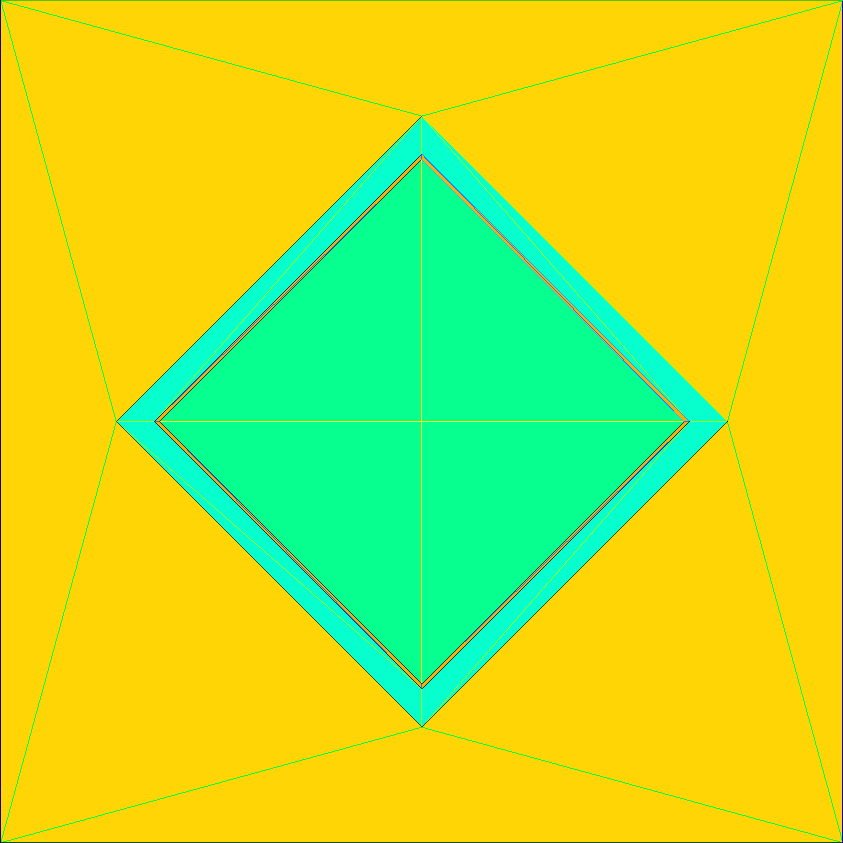
\includegraphics[width=0.5\textwidth]{chapters/tutorials/figures/beavrs_2d_mesh.png}
  \caption{2D Coarse Mesh for BEAVRS problem}
  \label{fig:beavrs_2d_mesh}
\end{figure}

This tutorial first explains how a tetrahedral mesh is created for the BEAVRS problem, then the cross sections data input is discussed, and finally the standard input to \ac{THOR} is covered.
The input files discussed below for the BEAVRS tutorial are located in:
\begin{verbatim}
    >> <thor_dir>/THOR/examples/tutorials/BEAVRS
\end{verbatim}

\subsection{BEAVRS Mesh}\label{ch:tuts:sec:beavrs:ssec:mesh}

The workflow described here is suitable if the user has access to a compatible version of \href{https://gmsh.info/}{Gmsh}.
Any version 4 Gmsh should work, but the example specifically performed here was done using Gmsh version 4.10.1.

Begin by navigating to the location of the BEAVRS Gmsh geometry files, which are found in:
\begin{verbatim}
  <thor_dir>/THOR/examples/tutorials/BEAVRS/mesh_create/
\end{verbatim}
Opening the file geometry file \verb"3d_beavrs.geo" in a text editor, it can be observed that the model is created by extruding a 2D BEAVRS fuel pin cell 50 cm in the axial direction.
For more details on creating original Gmsh inputs, see the \href{https://gmsh.info/doc/texinfo/gmsh.html}{Gmsh reference manual}.

Open \verb"3d_beavrs.geo" in Gmsh and run the ``3D'' command from the ``Mesh'' dropdown menu under ``Modules''.
The mesh should be generated and now become visible in the \ac{GUI}.
Now, select the ``Save'' command from the same ``Mesh'' dropdown to save the generated mesh to \verb"3d_beavrs.msh".
This mesh may be compared to the provided \verb"3d_beavrs_msh.ref", however they may differ slightly if the versions differ or if optimization of the mesh is employed.

The gmsh file \verb"3d_beavrs.msh" is converted to \ac{THOR}'s native mesh format by executing OpenMeshConverter with the command line:
\begin{verbatim}
  >> <thor_dir>/THOR/pre-processors/OpenMeshConverter/OpenMeshConverter.exe
      3D_beavrs.msh -bc 1 1 1 1 1 0
\end{verbatim}
Note that since we are modeling a 100 cm long system but the mesh is only extruded 50 cm, we make the -z boundary condition reflective since it should be axially symmetric anyway.
Also, since we are modeling an infinite lattice, the -x, +x, -y, and +y boundaries are also all reflective.
After successful completion of the conversion, the following printout should appear:
\begin{verbatim}
----------------------- Reading in gmsh:
Progress:***********************************************************************
----------------------- Calculating Adjacencies:
Progress:***********************************************************************
----------------------- Outputting thrm file:
Progress:***********************************************************************
----------------------- Calculating volumes:
Progress:***********************************************************************
Region 1 tets: 48
Region 1 volume:   1.5380515239999996E+01
Region 2 tets: 96
Region 2 volume:   6.2348501000000378E-01
Region 3 tets: 96
Region 3 volume:   4.8991837499999944E+00
Region 4 tets: 96
Region 4 volume:   5.8456657280000144E+01
Total number of tets: 336
Total system volume:   7.9359841279999927E+01
--------------------------------------------------------------------------------
--------------------------------------------------------------------------------
--------------------------------------------------------------------------------
------------------------- OpenMeshConverter successful -------------------------
----------------------- Output written to 3D_beavrs_out.thrm
\end{verbatim}

The file \verb"3D_beavrs_out.thrm" should result from this execution for use by THOR.
This mesh may be compared to the provided \verb"3D_beavrs_thrm.ref", which it should match if \verb"3D_beavrs.msh" matches \verb"3D_beavrs_msh.ref".
As with previous tutorials, the meshed volumes do not match the expected volumes.
This concludes the mesh generation step for this tutorial.

% \subsection{Cross section data}

The user should now move \verb"3D_beavrs_out.thrm" to the input file location
\begin{verbatim}
  <thor_dir>/THOR/examples/tutorials/BEAVRS/
\end{verbatim}
and navigate there to continue the tutorial.


The \ac{THOR} cross section file for the BeRP benchmark is provided by \verb"berp.xs".
\ac{THOR} uses a custom cross section format that is explained in detail in Section~\ref{ch:inp:sec:xsfile}.

At the end of Section~\ref{ch:tuts:sec:beavrs:ssec:mesh}, it was stated that there was a discrepancy in the volume of the BEAVRS mesh regions compared to the original problem.
To preserve material mass, the cross sections must be altered.
For this tutorial, this density factor adjustment is provided by \verb"3D_beavrs.dens"

\subsection{THOR input file and executing THOR}

The \ac{THOR} input file is \verb"3D_beavrs.inp".
\ac{THOR} uses a keyword-based input that is listed in Section~\ref{ch:inp:sec:stdinput}.
Upon running \ac{THOR}, a verbose form of the input will always be echoed, and ignored parameters will be highlighted as such.
\begin{verbatim}
problem_type          keig
keigsolver            pi
lambda                0
piacc                 none
kconv                 1e-7
innerconv             1e-8
outerconv             1e-7
maxinner              4
maxouter              50000
pnorder               1
mesh                  3D_beavrs_out.thrm
density_factor        3D_beavrs.dens
xs                    3D_beavrs.xs
qdtype                levelsym
qdorder               8
region_map            1 1
                      2 2
                      3 3
                      4 4
vtk_flux_out yes
vtk_mat_out yes
\end{verbatim}

The BEAVRS tutorial is solved with \ac{THOR} via the command line:
\begin{verbatim}
  >> <thor_dir>/THOR/thor-1.0.exe 3d_beavrs.inp
\end{verbatim}

Completion of execution of the BEAVRS tutorial is indicated by the printout:
\begin{verbatim}
--------------------------------------------------------
  Execution of THOR completed successfully
--------------------------------------------------------
\end{verbatim}

\ac{THOR} creates an output file, \verb"3d_beavrs_out.csv", that will report the computed $k_{eff}$ eigenvalue as 1.10297, and should match with \verb"3d_beavrs_out_csv.ref"

A plot of the group 25 flux for a slice along the axial direction using ParaView 5.10.0 for this run is shown in Figure~\ref{fig:beavrs_3d_g=25}.
\begin{figure}[th]
  \center
  
\includegraphics[width=1.0\textwidth]{chapters/tutorials/figures/beavrs_3d_g=25.png}
  \caption{Group 25 flux for BEAVRS tutorial.}
  \label{fig:beavrs_3d_g=25}
\end{figure}

The results can be improved by increasing the refinement of the mesh.
This can be achieved by reducing the mesh size parameter in the \verb"3D_beavrs.geo" file, that variable is \verb"runsize" which can be seen is set to 2.